%(BEGIN_QUESTION)
% Copyright 2011, Tony R. Kuphaldt, released under the Creative Commons Attribution License (v 1.0)
% This means you may do almost anything with this work of mine, so long as you give me proper credit

Dette nivåreguleringssystemet for vannfilter ser ut til å ``sykle'', med nivå som oscillerer over og under setpunkt over tid. Operatørene tilkaller deg og en annen tekniker for diagnose:

$$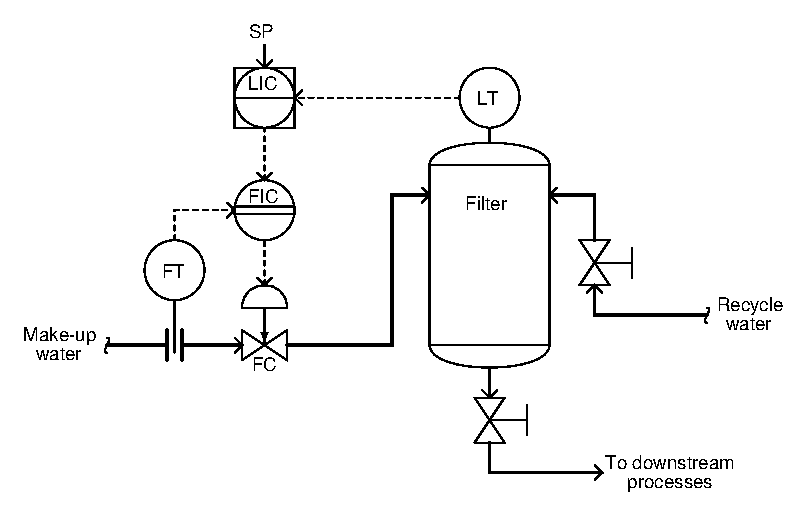
\includegraphics[width=15.5cm]{i00395x01.eps}$$

Teknikeren du jobber med setter LIC i manuell modus og ser på nivåtrendene på nytt. For hvert mulig testresultat under, angi {\bf ett} spesifikt problem som kan forårsake resultatet. Vær så konkret som mulig:

\vskip 10pt

\noindent
{\bf Mulig resultat 1} -- {\it Nivåsyklingen stopper} -- angi ett spesifikt problem som kan gi dette:

\vskip 100pt

\noindent
{\bf Mulig resultat 2} -- {\it Nivåsyklingen fortsetter} -- angi ett spesifikt problem som kan gi dette:

\underbar{file i00395}
%(END_QUESTION)





%(BEGIN_ANSWER)

Gi 5 poeng for {\it ett} spesifikt problem per testresultat.

\vskip 10pt

\noindent
{\bf Mulig resultat 1} -- {\it Nivåsyklingen stopper:}

\begin{itemize}
\item{} Ett spesifikt problem som kan gi dette:
\begin{itemize}
\item{} For mye integralvirkning i LIC
\item{} For mye derivatvirkning i LIC
\item{} LT sender ustabile strømsignaler
\end{itemize}
\end{itemize}

\noindent
{\bf Mulig resultat 2} -- {\it Nivåsyklingen fortsetter:}

\begin{itemize}
\item{} Ett spesifikt problem som kan gi dette:
\begin{itemize}
\item{} For mye integralvirkning i FIC
\item{} Ventilstiction (hysterese)
\item{} Ustabil ventilposisjonerer
\item{} Syklisk belastning i prosessen
\end{itemize}
\end{itemize}

%(END_ANSWER)





%(BEGIN_NOTES)

{\bf Denne oppgaven er ment for eksamen og ikke for arbeidsark!}.

%(END_NOTES)
